\documentclass[serif,envcountsect,table,t]{beamer}%, handout
\usepackage{amsmath, animate, hyperref, subcaption, tikz, multirow, pdfpages}
\usetheme{CambridgeUS}
\usecolortheme{wolverine}
\usecolortheme{orchid}
\setbeamertemplate{navigation symbols}{}
\graphicspath{{../figures/}}
\addtobeamertemplate{frametitle}{}{\vspace{-3mm}} % reduce top space
%%%%----------------------------------------------------------
\begin{document}
\title[Regression]{Pre College Summer - Data Science\\
Correlation and Regression}
\author[Bar, Wang]{Haim Bar, HaiYing Wang}
\date[]{}
\institute[UConn]{\normalsize University of Connecticut}
%%%% -------------------------------------------------
\begin{frame}[noframenumbering] \titlepage \end{frame}
%%%% -------------------------------------------------
\section{Correlation}
\begin{frame}{Sample Correlation Coefficient}
  The {\it sample correlation coefficient, $r$}, measures the strength and direction of linear association between two variables $x$ and $y$.
    \begin{itemize}
    \item $r$ is dimensionless and $-1\le r\le 1$, always;
  \item If $r>0$, the larger $r$ is, the stronger the {\it positive\/}
    association.
  \item If $r<0$, the larger $|r|$ is, the stronger the {\it
      negative\/} association.
  \item If $r\approx 0$, there is little linear association.
  \end{itemize}
  \begin{center}
    \begin{tabular}{cccc}
      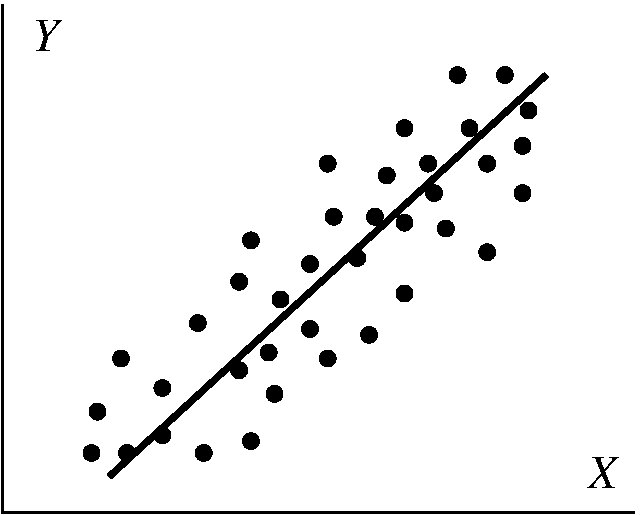
\includegraphics[scale=.25]{cc-r=1.pdf}\!\!&\!\!
      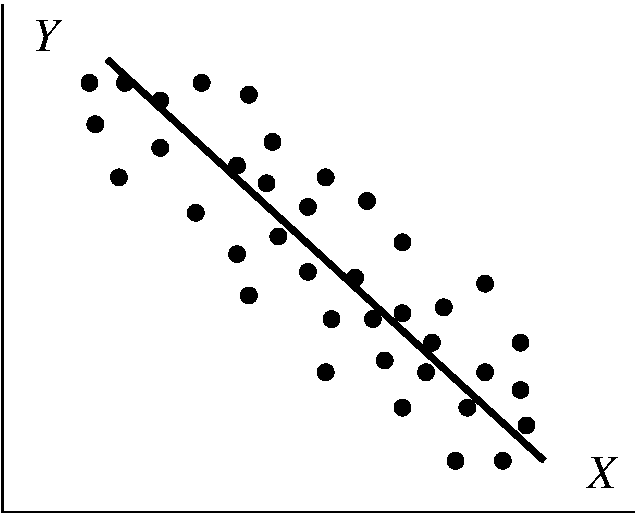
\includegraphics[scale=.25]{cc-r=-1.pdf}\!\!&\!\!
      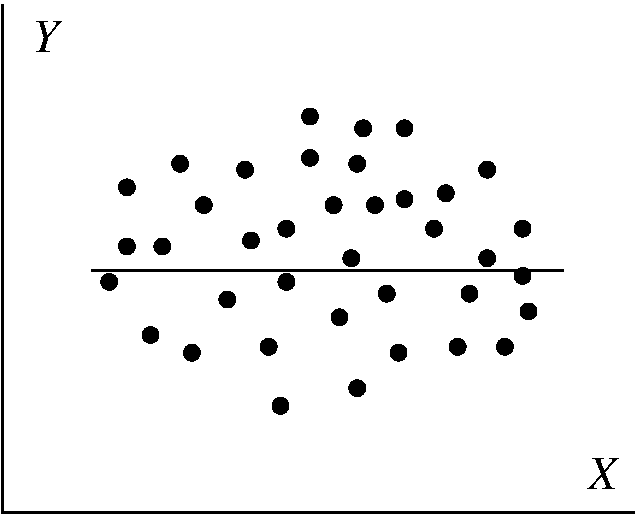
\includegraphics[scale=.25]{cc-r=0.pdf}\!\!&\!\!
      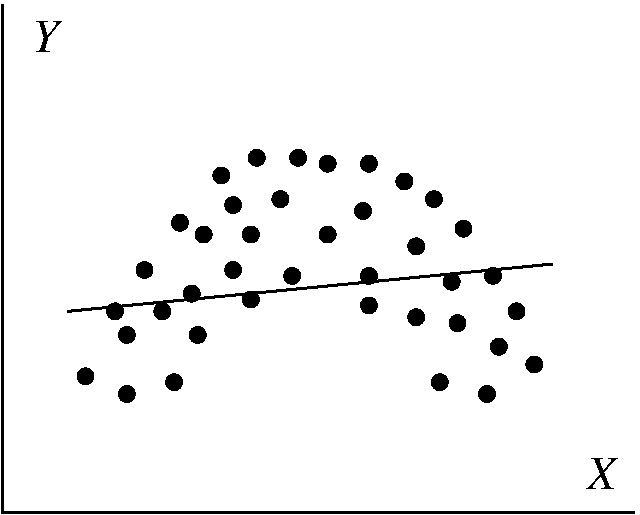
\includegraphics[scale=.25]{cc-nl.pdf}\\
    \begin{minipage}{2.4cm}\flushleft
      $r\approx 1$: strong positive association
    \end{minipage} &
    \begin{minipage}{2.4cm}\flushleft
      $r\approx -1$: strong negative association
    \end{minipage} &
    \begin{minipage}{2.4cm}\flushleft
      $r\approx 0$: no linear association
    \end{minipage} &
    \begin{minipage}{2.4cm}\flushleft
      $r\approx 0$: no linear association
    \end{minipage}
  \end{tabular}\\[2em]
    Correlation coefficient as a measure of association
  \end{center}
  \end{frame}
%%%% ------------------------------------------------
\begin{frame}
  \begin{center}
    \animategraphics[% autoplay,
    loop,controls,height=7cm]
    {3}{corr_seq}{0}{20}\protect
  \end{center}
\end{frame}
%%%% -------------------------------------------------
\section{Regression}
\begin{frame}{Body fat measurement}
  The most accurate and precise method of determining \%Body Fat is
hydrostatic weighing.
  It requires to submerse individuals in a tub of water and weigh them (hopefully before drowning).
  \begin{center}
    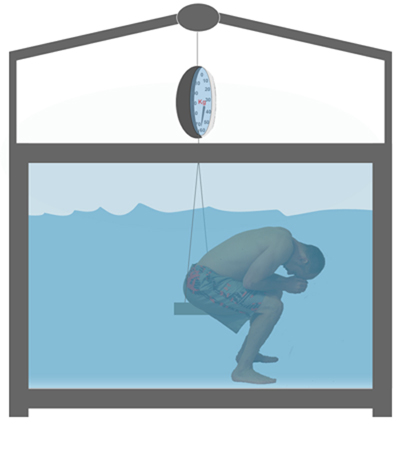
\includegraphics[width=0.5\textwidth]{huw.png}
  \end{center}
\end{frame}
%%%% -------------------------------------------------
\begin{frame}{Linear regression for body fat measurement}
  \begin{itemize}
  % \item A measure of health for an individual is \%Body Fat.
  % \item Unfortunately, the most accurate and precise method of determining body fat content is hydrostatic weighing.
  % \item It requires to submerse an individual in a tub of water and weigh them (hopefully before drowning).
  \item Since underwater weighing is inconvenient and unpleasant for the subject, researchers have attempted to use a number of convenient body measurements to estimate \%body fat.
  \item One model found by the researchers has the following inputs:
  \end{itemize}
  \begin{align*}
    BodyFat \approx  -6.22 & + 0.18\text{Age} + 0.10\text{Weight} \\
              & + 0.51\text{Chest} - 3.02\text{Wrist} + 0.07\text{BMI}
  \end{align*}
\end{frame}
%%%% -------------------------------------------------
\begin{frame}{Simple Linear Regression Model}
  \begin{equation*}
    y_i=\beta_0+\beta_1x_i+\varepsilon_i
  \end{equation*}
  \begin{itemize}
  \item $y_i$: response or dependent variable
  \item $x_i$: regressor or covariate
  \item $\varepsilon_i$: independent random error $\sim N(0,\sigma^2)$
  \item $\beta_0$: intercept parameter
  \item $\beta_1$: slope parameter (the amount of change in $y_i$ for
    per unit of change in $x_i$)
  \end{itemize}\-\\
   Here $\beta_0$ and $\beta_1$ are unknown and need to be estimated from data.
\end{frame}
%%%% -------------------------------------------------
\begin{frame}{Systolic blood pressure vs age}
  We want to study the relationship between systolic blood pressure ($y$) and age ($x$) using a sample of 30 individuals. The data is listed below.
  \begin{center}
    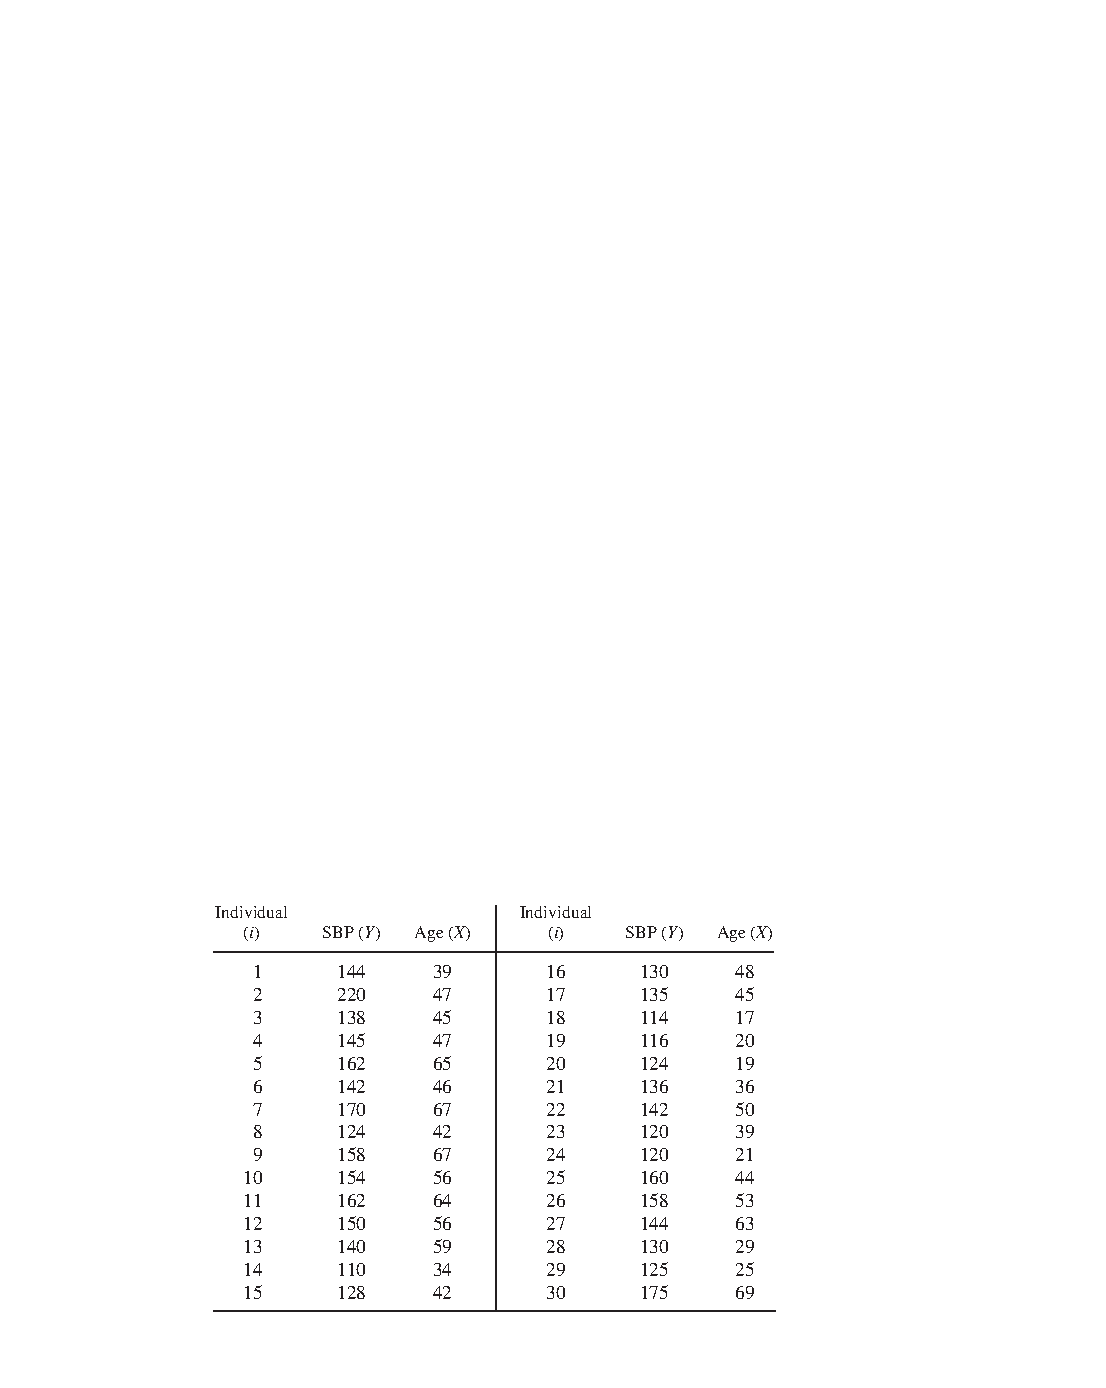
\includegraphics[width=0.7\textwidth]{table5-1.pdf}
\end{center}
\end{frame}
%%%% -------------------------------------------------
\begin{frame}[plain]{Least Squares estimate}
  \begin{center}\-\\[-3mm]
    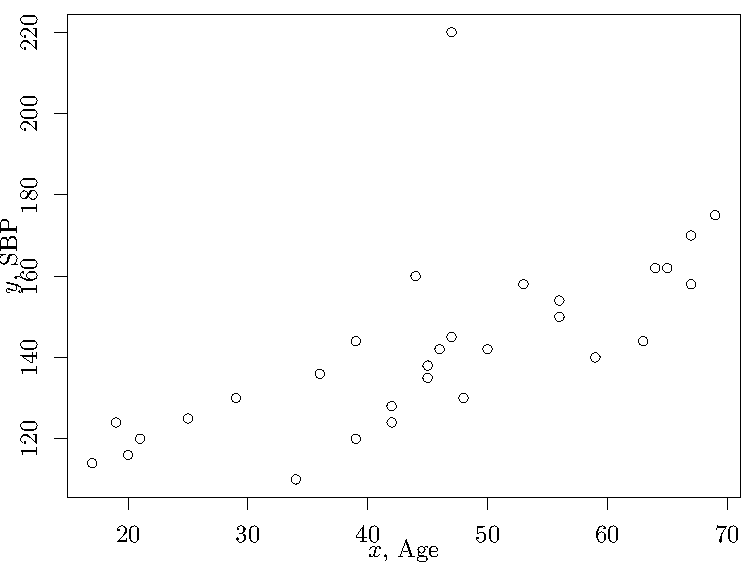
\includegraphics[width=0.95\textwidth]{LeastSquares.pdf}
  \end{center}
\end{frame}
{\setbeamercolor{background canvas}{bg=}
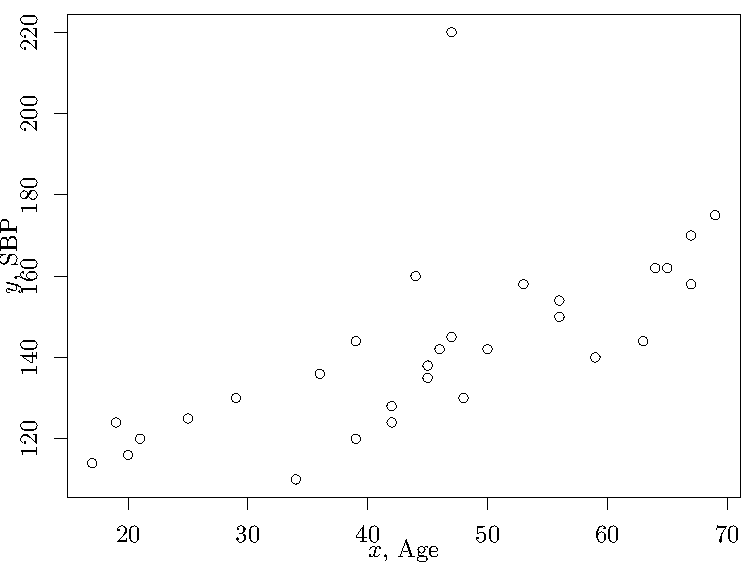
\includepdf[pages={1-5}]{LeastSquares.pdf}}
%%%% -------------------------------------------------
\begin{frame}{The least squares line}
  The line that minimizes the total error squares is:
  \begin{equation}
    \hat{\beta}_1 =
    \frac{\sum_{i=1}^n (x_i - \bar x)(y_i - \bar y)}
    {\sum_{i=1}^n (x_i - \bar x)^2}, \qquad
    \hat{\beta}_0 = \bar y - \hat{\beta}_1 \bar x.
  \end{equation}
 The regression line is $\hat y = \hat{\beta}_0 + \hat{\beta}_1 x$, and it minimize
 \begin{equation}
   \sum_{i=1}^n(y_i - \hat y_i)^2.
 \end{equation}

The distributions of $\hat{\beta}_0$ and $\hat{\beta}_1$ are (asymptotically) normal. 
\end{frame}
%%%%----------------------------------------------------------
\begin{frame}{Correctness v.s. usefulness}
  \Huge
  ``All models are wrong, but some are useful.'' -- George E. P. Box
\end{frame}
% %%%%----------------------------------------------------------
% \begin{frame}{}
% \end{frame}
% %%%% ----------------------------------------------------------
\end{document}
